%----------------------------------------------------------------------------------------
%	SECTION 1.1
%----------------------------------------------------------------------------------------

\section{Quotient Groups.}
\label{section1}

\begin{definition}
    Let $G$ and $H$ be groups and let $\phi:G \rightarrow H$ be a homomorphism
    of $G$ into  $H$. We define the \textbf{fiber} of $\phi$ over an element $h
    \in H$ to be the preimage of  $h$ under  $\phi$, i.e.  $\inv{\phi}(h)=\{g
    \in G : \phi(g)=h\}$.
\end{definition}

\begin{figure}[h]
    \centering
    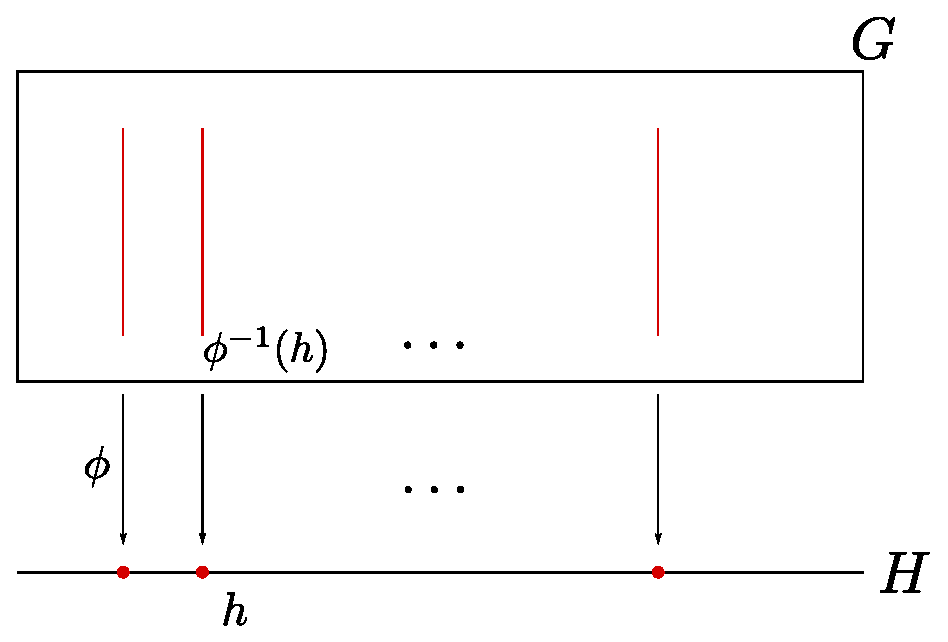
\includegraphics[scale = 0.5]{Figures/Chapter3/fibers.eps}
    \caption{The fibers of the elements of $H$ represented as vertical lines.}
    \label{fig_3.1}
\end{figure}

We can immediately define a special fiber for any homomorphisms.

\begin{definition}
    Let $G$ and  $H$ be groups and let  $\phi:G \rightarrow H$ be a homomorphism
    of $G$ into  $H$. We define the \textbf{kernel} of $\phi$ to be the fiber
    $\inv{\phi}(e')$ where $e'$ is the identity of  $H$. That is:
    \begin{equation}
        \ker{\phi}=\{g \in G : \phi(g)=e'\}
    \end{equation}
\end{definition}

\begin{lemma}\label{3.1.1}
    Let $G$ and  $H$ be groups and let  $\phi:G \rightarrow H$ be a hmomorphism
    of $G$ into  $H$. Then $\ker{\phi} \leq G$, and $\phi(G) \leq H$.
\end{lemma}
\begin{proof}
    We have that $\phi(e)=e'$ and for any $a,b \in \ker{\phi}$, that
    $\phi(ab)=\phi(a)\phi(b)=e'$, and that $\phi(\inv{a})=\inv{\phi(a)}=e'$.
    This makes $e',ab, \inv{a} \in \ker{\phi}$.
\end{proof}

\begin{example}\label{3.1}
    Take $\phi:\Z \rightarrow n\Z$ for any $n \in \Z$, defined by the rule  $a
    \rightarrow x^a$. Then $\phi(a+b)=x^{a+b}=x^ax^b=\phi(a)\phi(b)$. So $\phi$
    is a homomorphism of  $\Z$ onto $n\Z$, moreover, it is a homomorphism of
    $\Z$ onto  $\nZ$. Then, for any $x^a \in n\Z$, the fiber of $\phi$ under
    $x^a$ can be computed to be  $\inv{\phi}(x^a)=\{m \in \Z : m \equiv a
    \mod{n}\}$, which defines an equivalence class under congruence modulo $n$,
     $\equiv_n$ Thus, since $\phi$ is onto, $\inv{phi}(H)=\faktor{\Z}{n\Z}$.
\end{example}

This motivates the following results.

\begin{theorem}\label{3.1.2}
    Let $\inv{\phi}(H)$ be the set of all fibers of $\phi$ under elements of
    $H$, and define the operation $\inv{\phi}(a)\inv{\phi}(b)=\inv{\phi}(ab)$.
    Then $\inv{\phi}(H)$ forms a group under this operation.
\end{theorem}
\begin{proof}
    Let $\inv{\phi}(a)$ and $\inv{\phi}(b)$ be fibers of  $\phi$ under  $a$ and
     $b$ re spectively. Then for $g \in \inv{\phi}(a)$ and  $g' \in
     \inv{\phi}(b)$, we have  $\phi(gg')=\phi(g)\phi(g')=ab$, so that $gg' \in
     \inv{\phi}(ab)$, so this ensures that the operation is well defined.
     Moreover, we have that $\inv{\phi}(H)$ satisfies associativity because of
     the associativity of  $H$.

     Notice, then that  $\inv{\phi}(e)$ is the identity, as
     $\phi(gg_e)=\phi(g)\phi(g_e)=ae=a=ea=\phi(g_e)\phi(g)=\phi(g_eg)$, where $g
     \in \inv{\phi}(a)$ and $g_e \in \inv{\phi}(e)$. Similarly, we find that
     $\inv{\phi}(\inv{a})$ is the inverse of $\inv{\phi}(a)$ of $\inv{\phi}(H)$.
\end{proof}

\begin{definition}
    Let $G$ and  $H$ be groups, and let  $\phi:G \rightarrow H$ be a homomorphsm
    with $\ker{\phi}=K$. We deine the \textbf{quotient group} of $G$
    \textbf{mod} $K$ to be the group $\faktor{G}{K}$ of all fibers of $\phi$
    under elements of $K$.
\end{definition}

\begin{lemma}\label{3.1.3}
    Let $\phi$ be a homomorphism defined on a group  $G$ with  $\ker{\phi}=K$.
    Then for any fiber $\inv{\phi(a)} \in \faktor{G}{K}$, $a \in K$. we have
    for any $u \in \inv{\phi}(a)$, that $\inv{\phi}(a)=\{uk : k \in K\}$ and
    $\inv{\phi}(a)=\{ku : k \in K\}$.
\end{lemma}
\begin{proof}
    Let $uK=\{uk : k \in K\}$. Then since $\phi(u)=a$, for any $k \in K$, we
    have  $\phi(uk)=\phi(u)\phi(k)=ae=a$, making $uk \in \inv {\phi}(a)$. On the
    other hand, for some other $x \in \inv{\phi}(a)$, let $k=\inv{u}x$. Then
     $\phi(k)=\phi(\inv{u})\phi(x)=\inv{\phi(u)}\phi(x)=\inv{a}a=e'$, so $k \in
     K$. Then  $x=uk$, this  $x \in uK$. This makes  $\inv{\phi}(a)=uK$. The
     second assertion follows similarly.
\end{proof}

\begin{definition}
    Let $G$ be a group, and let  $H \leq G$. For any  $g \n G$, we define the
     \textbf{left} and \textbf{right cosets} of $H$ in $G$ to be the sets
     $gH=\{gh : h \in h\}$ and $Hg=\{hg : h \in h\}$, respectively.
\end{definition}
